%%%%%%%%%%%%%%%%%%%%%%%%%%%%%%%%%%%%%%%%%
% "ModernCV" CV and Cover Letter
% LaTeX Template
% Version 1.11 (19/6/14)
%
% This template has been downloaded from:
% http://www.LaTeXTemplates.com
%
% Original author:
% Xavier Danaux (xdanaux@gmail.com)
%
% License:
% CC BY-NC-SA 3.0 (http://creativecommons.org/licenses/by-nc-sa/3.0/)
%
% Important note:
% This template requires the moderncv.cls and .sty files to be in the same 
% directory as this .tex file. These files provide the resume style and themes 
% used for structuring the document.
%
%%%%%%%%%%%%%%%%%%%%%%%%%%%%%%%%%%%%%%%%%

%----------------------------------------------------------------------------------------
%	PACKAGES AND OTHER DOCUMENT CONFIGURATIONS
%----------------------------------------------------------------------------------------

\documentclass[11pt,a4paper,sans]{moderncv} % Font sizes: 10, 11, or 12; paper sizes: a4paper, letterpaper, a5paper, legalpaper, executivepaper or landscape; font families: sans or roman

\moderncvstyle{classic} % CV theme - options include: 'casual' (default), 'classic', 'oldstyle' and 'banking'
\moderncvcolor{blue} % CV color - options include: 'blue' (default), 'orange', 'green', 'red', 'purple', 'grey' and 'black'

%\usepackage{lipsum} % Used for inserting dummy 'Lorem ipsum' text into the template

\usepackage[scale=0.82]{geometry} % Reduce document margins
%\setlength{\hintscolumnwidth}{3cm} % Uncomment to change the width of the dates column
%\setlength{\makecvtitlenamewidth}{10cm} % For the 'classic' style, uncomment to adjust the width of the space allocated to your name

\usepackage{multicol}

\usepackage{background}
\backgroundsetup{
scale=1,
angle=0,
opacity=.05,  %% adjust
contents={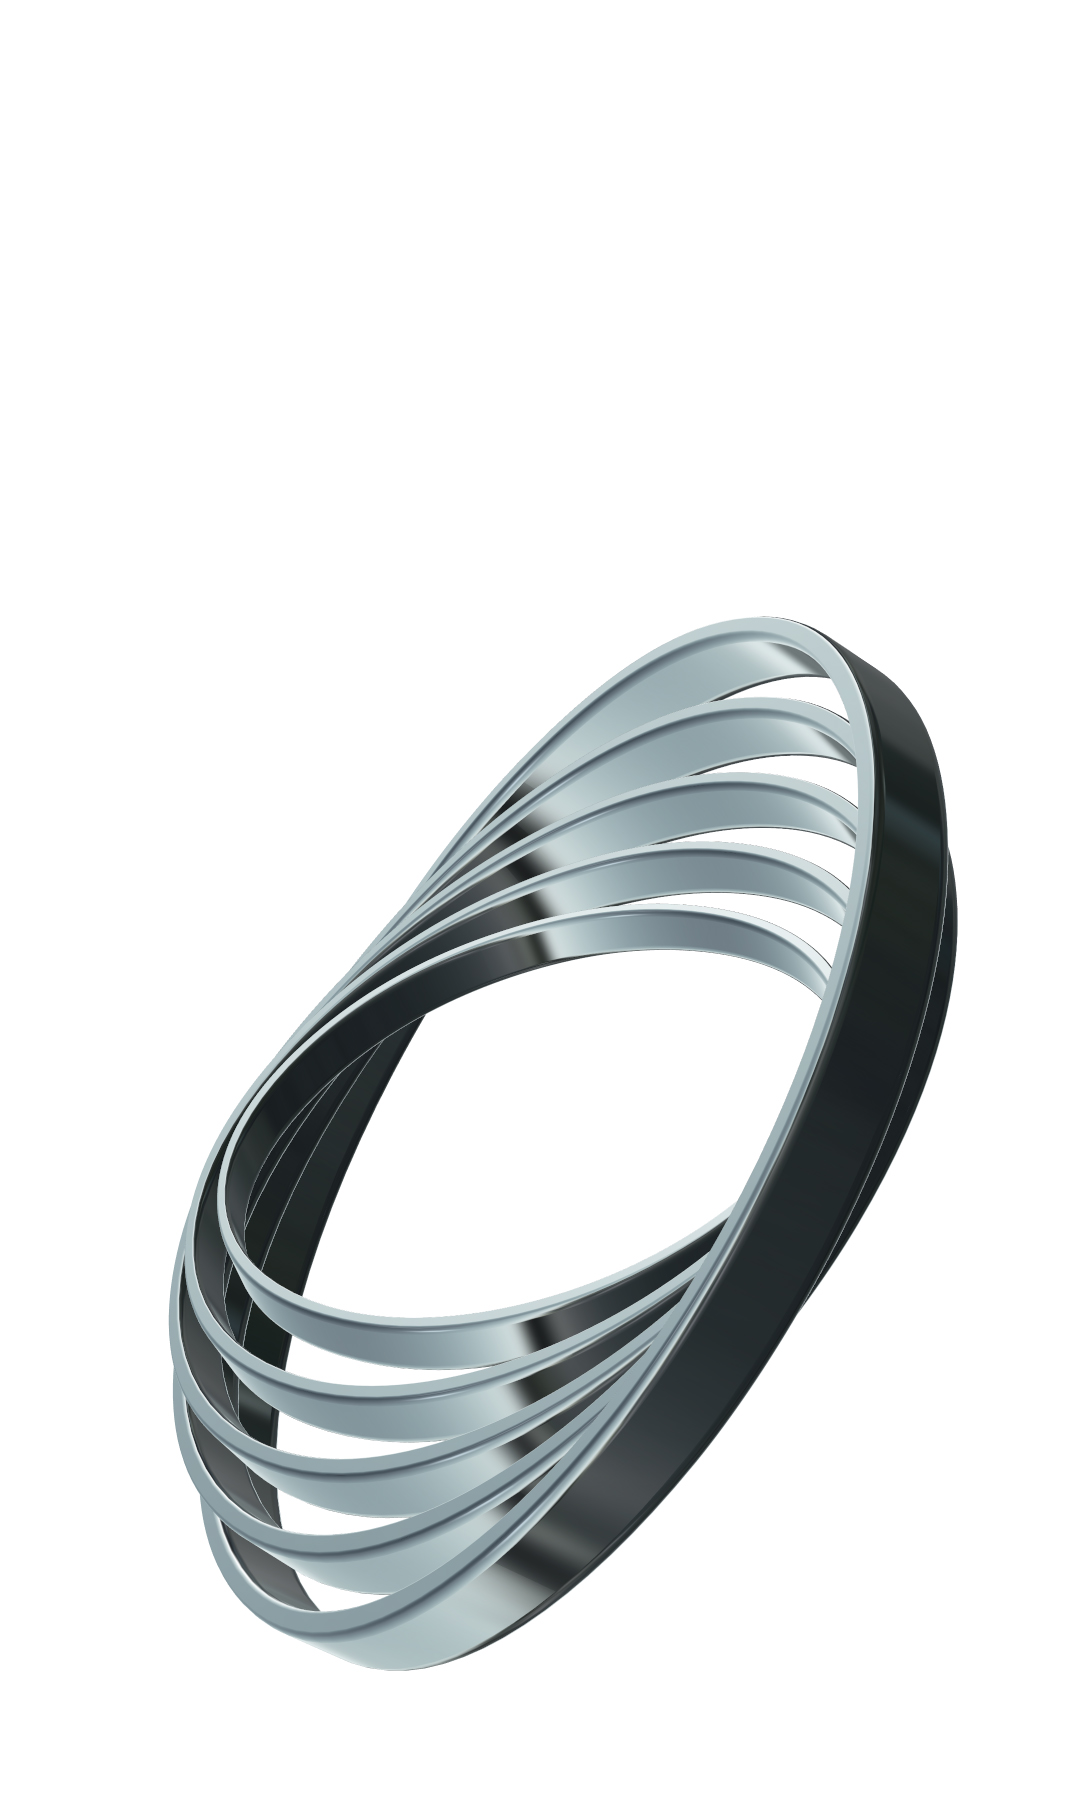
\includegraphics[trim={0 0 0 17cm},width=\paperwidth,height=\paperheight]{pictures/BG5.jpg}}
}
%----------------------------------------------------------------------------------------
%	NAME AND CONTACT INFORMATION SECTION
%----------------------------------------------------------------------------------------

\firstname{Antonius} % Your first name
\familyname{Torode} % Your last name

% All information in this block is optional, comment out any lines you don't need
\title{Active Secret Security Clearance\newline\newline https://torodean.github.io}
\address{Austin, TX 78759}{}
\mobile{517-512-3580}
%\phone{None}
\email{AWTorode@gmail.com}
%\homepage{https://torodean.github.io}{https://torodean.github.io} % The first argument is the url for the clickable link, the second argument is the url displayed in the template - this allows special characters to be displayed such as the tilde in this example
%\extrainfo{Contact via e-mail is best}
%\photo[70pt][0.4pt]{pictures/picture_me} % The first bracket is the picture height, the second is the thickness of the frame around the picture (0pt for no frame)
%\quote{}

%----------------------------------------------------------------------------------------

\begin{document}

\makecvtitle % Print the CV title

%----------------------------------------------------------------------------------------
%	Summary
%----------------------------------------------------------------------------------------

Exceptionally well organized and resourceful professional with more than 10 year’s experience, with a solid academic background, excellent analytical and problem solving skills, and able to handle multiple projects while producing high quality work. Experienced in software development and a strong working knowledge of algorithms and data structures.	

%----------------------------------------------------------------------------------------
%	SKILLS SUMMARY
%----------------------------------------------------------------------------------------

\section{Skills Summary}

\begin{multicols}{3}
	\begin{itemize}
	\item Problem-Solving
	\item Research \& Development
	\item Software Development
	\item Engineering
	\item Software Deployment
	\item GUI Design \& Development
	\item Security+ Certified
	\item Web Development
	\item Mathematics
	\item Technical Documentation
	\item End User Documentation
	\item Software Testing
	\end{itemize}
\end{multicols}

%----------------------------------------------------------------------------------------
%	COMPUTER SKILLS SECTION
%----------------------------------------------------------------------------------------

\section{Computer and Technology Summary}

\cvitem{Languages}{\textsc{c}++, \textsc{python}, \textsc{c}\#, \textsc{java}, \textsc{git},  \textsc{bash}, \textsc{cmake}, \textsc{php}, \textsc{root} \textsc{geant4}, \textsc{html}, \textsc{css}, \textsc{cad}, \LaTeX, Perforce, Qt, Eclipse, CLion, NetBeans, Cygwin, Makefiles, LabVIEW, Mathematica, TLS/SSL, Telnet, IBM MQ, Systemd, GDB}
\cvitem{Systems}{Microsoft Windows (all modern), Linux (Ubuntu, RedHat, Kali, Debian, CentOS, Fedora, Raspian, others), \textsc{Mac OS}, UNIX}
\cvitem{Software}{OpenOffice products, Microsoft Office Suite, Adobe (Premiere Pro, Illustrator, Photoshop, After Effects, Audition), TexStudio, DS9, Stellarium, Sony Vegas, Final Cut Studio, GIMP, PuTTY, Notepad++, FileZilla, VLC, OBS, Blender}

%----------------------------------------------------------------------------------------
%	WORK EXPERIENCE SECTION
%----------------------------------------------------------------------------------------

\section{Experience}

%\subsection{Vocational}

\cventry{2024--Pres}{Owner}{Torode On The Road, LLC.}{Austin, TX}{}{
	\begin{itemize}
		\item An multidisciplinary artisan and innovation startup.
		\item Specializing in custom carpentry, lumber work, integrated circuitry, handyman services, and innovative device design.
\end{itemize}}

\cventry{2019--Pres}{Engineering Scientist}{\textsc{Applied Research Laboratories}}{Austin, TX}{}{
	\begin{itemize}
		\item Programming and implementing new technologies used by satelite GPS systems. 
		\item Developed multiple applications for automating and improving the GPS network, systems, and development process.
		\item Managing and implementing system design structures via high and low level documentation.
		\item Training others in software skills, standards, best practices, and application development.
\end{itemize}}

\cventry{2019}{IT Helpdesk Specialist}{\textsc{Casey's}}{Des Moines, IA}{}{
	\begin{itemize}
		\item Computer, register, and other Casey's hardware/software troubleshooting and repair.
\end{itemize}}

%------------------------------------------------

\cventry{2017--2018}{Undergraduate Research Assistant}{\textsc{National Superconducting Cyclotron Laboratory}}{East Lansing MI}{}{
\begin{itemize}
\item Experimental nuclear astrophysics with a primary focus was with scintillator detectors and experimental setups to better understand nucleosynthesis. This involved designing, building, and testing detector systems and collecting data using photomultiplier tubes and the NSCL DAQ system.
\item I also performed calculations and simulations written in \textsc{python} and \textsc{c}++ for determining existing detector properties and new detector properties. 
\end{itemize}}

%------------------------------------------------

\cventry{Summer 2018}{LabVIEW Programmer}{\textsc{Michigan State University}}{East Lansing MI}{}{
\begin{itemize}
	\item Programming and documentation of experimental data acquisition systems for an advanced lab class at MSU for quantum physics (optical pumping) and superfluidity experiments by integrating National Instruments I/O devices to a computer system.
\end{itemize}}

%------------------------------------------------

\cventry{2016--2018}{Physics and Astronomy Computing Assistant}{\textsc{Michigan State University}}{East Lansing MI}{}{
\begin{itemize}
\item My responsibilities included managing and fixing any computer related problems that may arise while maintaining or improving efficiency within multiple departments. These included problems such as setting up experimental camera systems, restoring corrupted operating system files, recovering lost data, replacing damaged hardware, troubleshooting malfunctioning software and more.
\end{itemize}}

%------------------------------------------------

\cventry{Summer 2016}{Physics Teaching Assistant}{\textsc{Michigan State University}}{East Lansing MI}{}{
\begin{itemize}
\item A tutor and exam proctor for PHY 232C, an online course taught at MSU.
\item Assisting students in the understanding of concepts and problems via online and in person.
\end{itemize}}
	
%------------------------------------------------

\cventry{2013--2015}{CRLA Certified Math, Physics and Chemistry Tutor}{\textsc{Oakland Community College}}{Auburn Hills MI}{}{
\begin{itemize}
\item Tutor for fundamental concepts and ideas of mathematics, physics and chemistry.
\end{itemize}}

%------------------------------------------------

\cventry{Summer 2013}{Condensed Matter Physics Researcher}{\textsc{Oakland University}}{Auburn Hills MI}{}{
\begin{itemize}
\item Extensively studied Raman spectroscopy and graphite/graphene under high pressures.
\item Performed a Raman spectroscopy experiment on graphene using a diamond anvil cell. 
\item Designed and set up resistivity experiments to confirm spectroscopic findings.
\item Presented research in a professional and comprehensive manner in front of an audience.
\end{itemize}}

%------------------------------------------------

\cventry{2011--2013}{Data Research Analyst}{\textsc{CLRS, inc.}}{Southfield MI}{}{
\begin{itemize}
\item Performed Data analysis of different financial markets such as the GM commercial car market. 
\item In depth research of Las Vegas casino populations.
\item Improved business functionality and efficiency by optimizing data verification process.
\end{itemize}}

%------------------------------------------------

\cventry{2010--Present}{d0sag3-Films}{\textsc{Home Business}}{}{}{
\begin{itemize}
\item Graphic design and 3D modeling for film and animation industry. 
\item Contract work for Detroit In Focus and also many personal projects.
\end{itemize}}

%----------------------------------------------------------------------------------------
%	PUBLICATIONS \& PROJECTS
%----------------------------------------------------------------------------------------

\section{Peer Reviewed Publications}

%\cvitem{2018--Present}{See \url{https://torodean.github.io/projects.html\#publications}}
\cvitem{May 2023}{"High-pressure phase of cold-compressed bulk graphite and graphene nanoplatelets." Phys. Rev. B 107, 184102 - https://doi.org/10.1103/PhysRevB.107.184102}
\cvitem{Jan 2020}{"Extracting the Anharmonic Properties of the G-Band in Graphene Nanoplatelets." Journal of Physical Chemistry - 2020, 124, 8, 4835–4842 - https://doi.org/10.1021/acs.jpcc.9b10875}
\cvitem{Jan 2018}{"Software Development to Determine the Optimal Parameters of a Tape Transport System." Student Journal of Physics - International Version - Vol. 7. No. 1. Jan-March 2018 - Indian Association of Physics Teachers.}
\cvitem{Jun 2017}{"Exploration of the Quantum Casimir Effect." Student Journal of Physics - International Version - Vol. 6. No. 2. April-June 2017 - Indian Association of Physics Teachers.}

%\section{Other Publications and Projects}
%
%\cvitem{2018}{"Multiple Integrated Applications (MIA)." Program created for further development of application design. Contains mathematical functions, encryption algorithms, key code simulations, a comprehensive workout generation system, and more.}
%%\cvitem{Oct 2017}{"Characterizing a Tape Station and Beta Detector For Radioactive Isotope Beam Experiments." Conference Poster presented at the Fall Meeting of the Division of Nuclear Physics of the American Physical Society}
%\cvitem{2017}{"Generations of Nuclear Activity (GINA)." Program created for performing nuclear decay calculations for a new radioactive transport system at the NSCL.}
%\cvitem{2017}{"Local Operations Listing Agent (LOLA)." Program created for improved efficiency and computer database management at MSU.}
%%\cvitem{May 2017}{"The Antonius Cookbook." Self Published: Free culinary cookbook download. https://torodean.github.io/ACookbook.html}
%\cvitem{Nov 2016}{"Antonius' Handbook." Comprehensive reference of useful formulas, constants, units and definitions. Self Published Book (see homepage).}


%----------------------------------------------------------------------------------------
%	EDUCATION SECTION
%----------------------------------------------------------------------------------------

\section{Education}

\cventry{2018--2019}{Degree in Biblical Studies}{Ambassador Bible College}{Milford OH}{}{Theology and historical studies pertaining to the history and contents of the Bible and other religions.}
\cventry{2015--2018}{B.S., Physics, Mathematics (Dual Majors)}{Michigan State University}{East Lansing MI}{%\textit{GPA -- 3.8}
}{
\begin{itemize}
\item Graduated with an undergraduate physics degree and mathematics degree.
\item Nominated for and received the Lawrence W. Hantel Endowed Fellowship. 
\end{itemize}}
\cventry{2011--2014}{Undergraduate Studies}{Oakland Community College}{}{%\textit{GPA -- 3.7}
}{General studies as well as math/sciences up to and including Calculus III, Differential Equations, Engineering Physics II and General Chemistry II (4.0 in all).}
%\cventry{2008--2011}{High School}{Clarkston High School}{Clarkston MI}{AP Physics, AP Calculus, AP Computer Sciences, CSMTech (3 year advanced math, science and technology program).}  % Arguments not required can be left empty



%----------------------------------------------------------------------------------------
%	AWARDS SECTION
%----------------------------------------------------------------------------------------

%\section{Honors, Clubs, and Other Affiliations}
%
%\cvitem{2016-2018}{Michigan State University Dean's List}
%\cvitem{2017}{Lawrence W. Hantel Endowed Fellowship Fund, in Memory of Professor Donald J. Montgomery}
%\cvitem{2016-2017}{Regular Attendee of Physics, Astronomy, and Karate Clubs at Michigan State University}
%\cvitem{2015}{Member of the Phi Theta Kappa Honor Society}
%\cvitem{2011-2015}{Oakland Community College Dean's List}
%\cvitem{2010}{Member of the National Junior Classical League}

%----------------------------------------------------------------------------------------
%	COMMUNICATION SKILLS SECTION
%----------------------------------------------------------------------------------------

%\section{Communication Skills}

%\cvitem{2011--2012}{Composition I/II classes with various presentations}
%\cvitem{2013}{REU Condensed Matter Research presentation}

%----------------------------------------------------------------------------------------
%	LANGUAGES SECTION
%----------------------------------------------------------------------------------------

%\section{Languages}

%\cvitemwithcomment{English}{Mothertongue}{}
%\cvitemwithcomment{German}{Basic}{Basic words and phrases only}
%\cvitemwithcomment{Japanese}{Basic}{Basic words and phrases only}

%----------------------------------------------------------------------------------------
%	INTERESTS SECTION
%----------------------------------------------------------------------------------------

%\section{Interests and Hobbies}
%\cvitem{}{Mathematics, Chess, Chemistry,
%	Physics, Mathematics, Video Design, Computer Sciences, Health and Education, Technology}

%----------------------------------------------------------------------------------------
%	REFERENCES SECTION
%----------------------------------------------------------------------------------------

%\section{References}
%
%\cventry{2017--2018}{Artemis Spyrou}{Associate Professor of Physics, National Superconducting Cyclotron Laboratory}{Cyclotron, 640 S Shaw Ln, East Lansing, MI 48824}{spyrou@nscl.msu.edu (517)-908-7141}{Supervisor at NSCL.}
%\cventry{2016--2018}{Esther V. V. Reed}{MSU Information Technologist Departmental Support}{Biomed/Physical Science Building: 567 Wilson Road, Room 1209, East Lansing, MI 48824}{reed@pa.msu.edu (517)-884-5469}{Supervisor at Michigan State University.}
%\cventry{2013--2015}{Michael Robinson}{OCC Faculty}{739 S Washington Ave, Royal Oak, MI 48067}{mdrobins@oaklandcc.edu (248)-232-4438}{Employer at Oakland Community College.}
%\cventry{2011--2013}{Mitch Kanaan}{CLRS, inc. President/Owner}{29433 Southfield Road, Suite 106 Southfield, Michigan 48076}{mkanaan@clrsinc.com (248)-760-5316}{Employer at CLRS, Inc.}

%----------------------------------------------------------------------------------------
%	COVER LETTER
%----------------------------------------------------------------------------------------

% To remove the cover letter, comment out this entire block

%\clearpage

%\recipient{HR Department}{Corporation\\123 Pleasant Lane\\12345 City, State} % Letter recipient
%\date{\today} % Letter date
%\opening{Dear Sir or Madam,} % Opening greeting
%\closing{Sincerely yours,} % Closing phrase
%\enclosure[Attached]{curriculum vit\ae{}} % List of enclosed documents

%\makelettertitle % Print letter title

%\lipsum[1-3] % Dummy text

%\makeletterclosing % Print letter signature

%----------------------------------------------------------------------------------------

\end{document}
